% Documento do tipo artigo, com fonte tamanho 11
\documentclass[11pt]{article}

% Configura o tamanho do papel e das margens
\usepackage[
    a4paper,
    top=20mm,
    right=20mm,
    bottom=10mm,
    left=20mm
]{geometry}

% Suporte a caracteres acentuados
\usepackage[utf8]{inputenc}

% Configura o idioma para português do Brasil, incluindo suporte a hifenização
\usepackage[brazil]{babel}

% Melhora a renderização da fonte Computer Modern em PDFs modernos
\usepackage{lmodern}

% Melhora a codificação da fonte
\usepackage[T1]{fontenc}

% Permite a inclusão de imagens / PDF como imagem
\usepackage{graphicx}

% Permite cores por nome
\usepackage{xcolor}

% Permite personalizar listas
\usepackage{enumitem}

% Configure o \includegraphics a não emitir a seguinte mensagem de warning:
% PDF inclusion: multiple pdfs with page group included in a single page
\pdfsuppresswarningpagegroup=1

 % Remove a numeração das páginas
\pagestyle{empty}

% Começo do documento
\begin{document}

\begin{center}
UNIVERSIDADE FEDERAL DA PARAÍBA

CENTRO DE CIÊNCIAS EXATAS E DA NATUREZA

DEPARTAMENTO DE ESTATÍSTICA

DISCIPLINA: INFERÊNCIA I
\end{center}

\textbf{Docente:} Dra Tatiene Correia de Souza

\textbf{Discente:} Fabrício Barros Cabral -- 20230052696

\begin{center}
{\Large \textbf{Análise das Marcas de Café A e B para a CoffeeMax}}
\end{center}

\begin{enumerate}
    \item \textbf{Qual fornecedor tem teor de cafeína mais adequado em média?}

    A marca A possui, em média, aproximadamente 95,18\% mg [94,12;95,97] de
    cafeína por xícara, enquanto a marca B possui, em média, aproximadamente
    95,30\% mg [93,30;96,77]. Analisando estas médias com o intervalo de
    confiança de 99\% verificou-se que a média não varia para a marca A ou para
    a marca B. Também verificou-se que, em média, \textbf{não há evidência
    estatística de diferença significativa do teor de cafeína entre as marcas}.

    \item \textbf{Qual fornecedor apresenta maior consistência (menor
    variabilidade)?}

    \begin{figure}[h!]
        \centering
        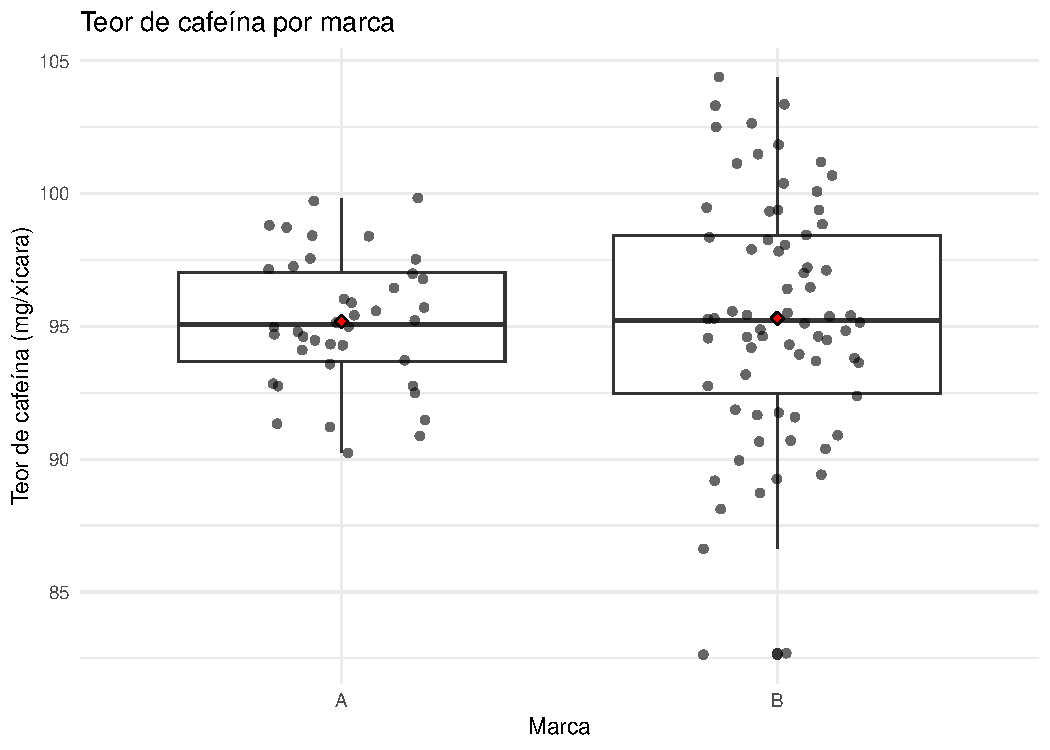
\includegraphics[scale=0.4]{plots/boxplot_cafeina_AB.pdf}
        \caption{Boxplot da variabilidade do teor de cafeína}
        \label{fig:boxplot-cafeina}
    \end{figure}

    A marca A possui variância de aproximadamente 9,09 $(mg)^2$ [4,09;10,04] por
    xícara de café, enquanto que a da marca B é de aproximadamente 21,51
    $(mg)^2$ [15,81;30,97]. Além disso, foi calculada a razão entre a variância
    do café da marca A e da marca B, e com o intervalo de confiança de 99\%,
    podemos afirmar que há uma diferença na variabilidade entre as marcas.
    Assim, concluímos que a marca B possui uma variabilidade maior que a marca A
    e, portanto, \textbf{a marca A apresenta maior consistência}.

    \item \textbf{Qual fornecedor é mais aceito pelos consumidores?}

    Conforme a pesquisa de opinião com 120 consumidores para cada marca, em que
    a marca A foi aprovada por 78 consumidores e a marca B foi aprovada por 69
    consumidores, foram analisadas as proporções com intervalo de confiança de
    99\% e concluímos que \textbf{não há diferença estatística significativa
    entre as proporções de aprovação entre as duas marcas de café}.

    \item \textbf{Recomendação final}

    Considerando as informações elencadas dos itens anteriores e o fato que a
    empresa \textbf{CoffeeMax} deseja lançar um \textit{blend} premium e,
    portanto, um café de melhor qualidade, \textbf{recomendamos a compra da
    marca A}, pois o café da marca A é mais previsível (consistente) do que o da
    marca B. Além disso, como a pesquisa de opinião com os consumidores não
    conseguiu (estatisticamente) distinguir qual o café é o mais aceito pelos
    consumidores, deve-se adotar um perfil conservador com relação à qualidade
    do café (menor variabilidade), pois o mesmo visa um público mais exigente
    com relação à consistência da qualidade da marca escolhida.
\end{enumerate}
\end{document}
